



\chapter{Bandpass Sampling}

Now we move to what we call bandpass sampling or higher order sampling. Before getting directly into the process, we talk first about bandpass signals in general, and how to represent them.

\begin{itemize}

\item Bandpass signal are encountered in RF application (communication and radar )


\item The amplitude spectrum is centered at a center frequency $f_c$

\item When a receiver process a transmitted signal, they don't process it in the bandpass form, they turn into what we call \tbi{equivalent low pass signal}, which is a \tbi{generalization of the idea of phasor}.

\end{itemize}

There are 3 ways of sampling in bandpass cases:

\begin{enumerate}
    \item Integer band positioning
    
    \item Non Integer Band positioning
    
    \item Quadrature sampling, which use IQ representation of a signal
    
\end{enumerate}


\section{Integer Band Positioning}

\todo{Integer Band Positioning}

\textit{To write it later}


\section{Non-Integer Band Positioning}

\todo{Non- Integer Band Positioning}

\textit{To write it later}


\newpage
\section{Quadrature Sampling}

Before, we review the concept of IQ representation.

\subsection{Review of Phasor Notation}

\underline{Phasor Idea:}\\

\begin{figure}[h]
\centering
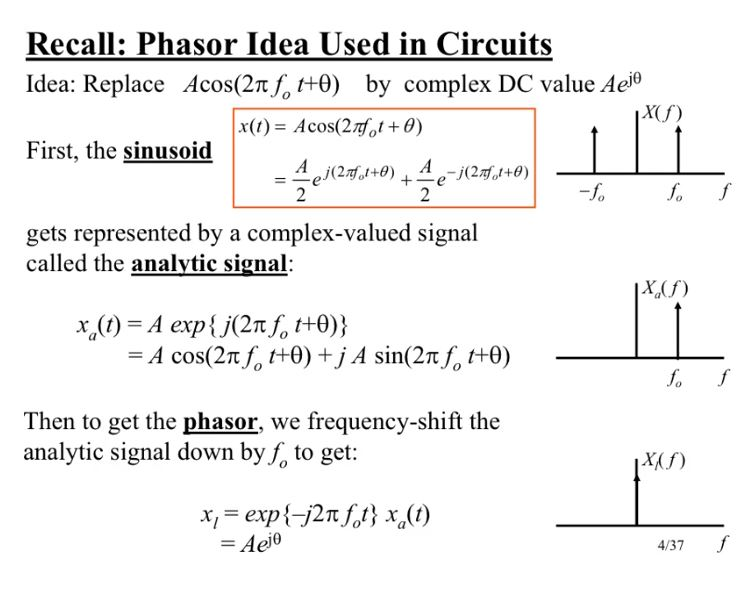
\includegraphics[width = 0.7\textwidth, frame]{Figures/Sampling/bandpass_to_lowpass_cosine}
\caption{Equivalent Low pass signal to a cosine signal}
\label{fig:Sampling:bandpass_to_lowpass_cosine}
\end{figure}

\begin{itemize}

\item We have some bandpass signal $x(t) \, = \, A \, \text{cos}\left(\, 2 \pi f_0 \, + \, \theta  \,\right)$

\item Using Euler formula, we obtain 2 dirac function at $f_0$ and $- f_0$

\item Turn the signal into analytically form by suppressing the negative frequency component at $-f_0$

\item Then we shift the component at $+f_0$ to dc by multiplying by $\text{exp}\left(\, -j 2 \pi f_0 t \,\right)$

	\begin{itemize}
	\item The obtained signal is called $x_{low-pass}$ which is \tbi{complex value signal}
	\end{itemize}

\end{itemize}


\newpage
\subsection{Equivalent Low Pass Signal}

We can generalize this idea into a general bandpass signal, as shown in \autoref{fig:Sampling:bandpass_to_lowpass_general}.


\begin{figure}[h]
\centering
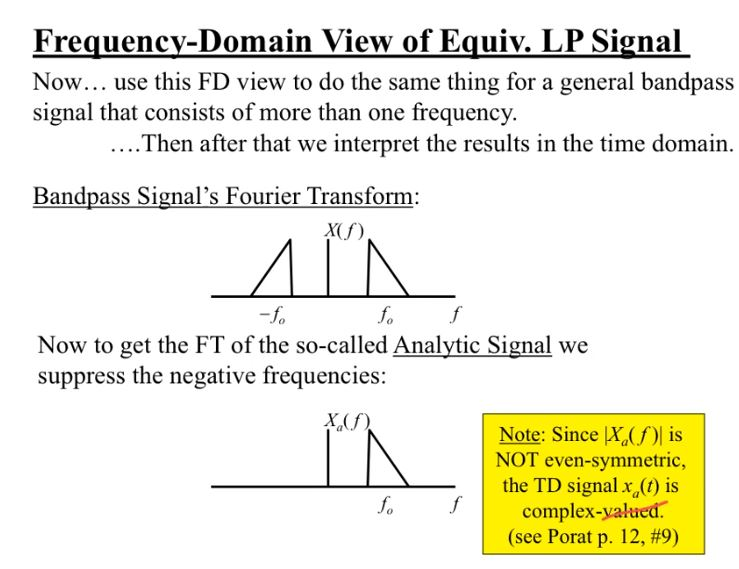
\includegraphics[width = 0.7\textwidth, frame]{Figures/Sampling/bandpass_to_lowpass_general}
\caption{Equivalent Low pass signal to a general bandpass signal}
\label{fig:Sampling:bandpass_to_lowpass_general}
\end{figure}


\begin{itemize}

\item Be aware that since $X_{\text{analyticall}}(f_c)$ has no symmetry around the y-axis, this means that $x_{\text{analyticall}}(t)$ is \tbi{complex signal}

\end{itemize}

\newpage
So we start by a real value bandpass signal, and turn it into a complex value low pass signal.  \\

A system point of view for implementing the suppression of the negative frequency part is shown in \autoref{fig:Sampling:hilbert_bandpass_lowpass}, where $H(f_c)$ is known as Hilbert transform.

\begin{figure}[h]
\centering
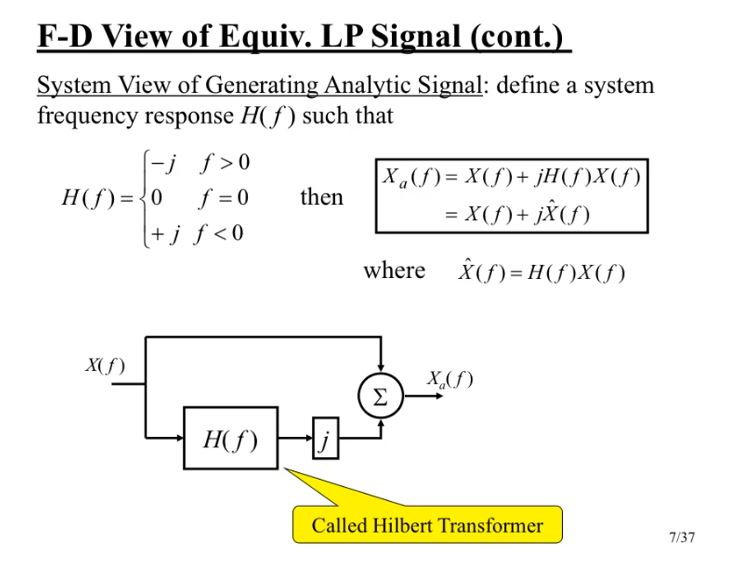
\includegraphics[width = 0.7\textwidth, frame]{Figures/Sampling/hilbert_bandpass_lowpass}
\caption{System point of view to implement the suppression of negative frequency spectrum}
\label{fig:Sampling:hilbert_bandpass_lowpass}
\end{figure}


\begin{itemize}

\item We apply Hilbert transform to $X_{\text{band-pass}}(f_c)$, then add the output with the original signal $X_{\text{band-pass}}(f_c)$

\end{itemize}

\newpage
After we obtain $X_{\text{analyticall}}(f_c)$ which is a complex signal, we shift down the frequency spectrum and hence we obtain $X_{\text{low-pass}}(f_c)$  as shown in \autoref{fig:Sampling:shift_frequency_down}. 

\begin{figure}[h]
\centering
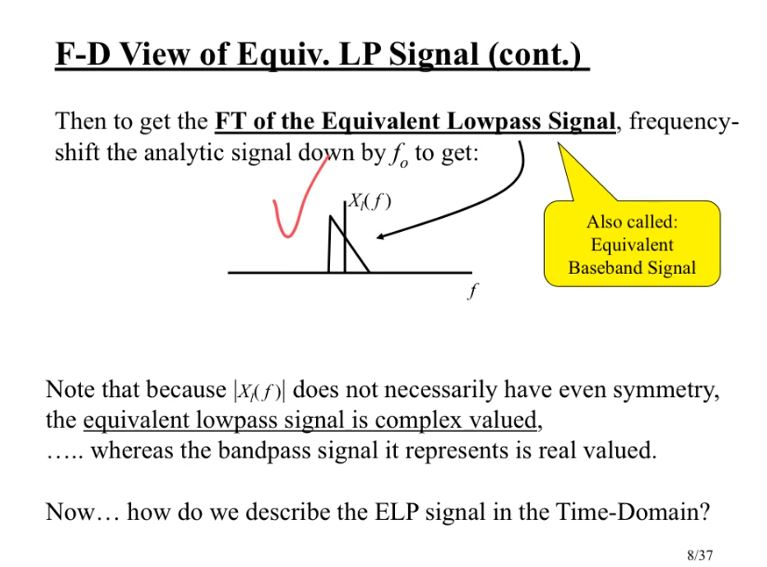
\includegraphics[width = 0.7\textwidth, frame]{Figures/Sampling/shift_frequency_down}
\caption{Shifting down the frequency spectrum of $X_{\text{analyticall}}(f_c)$}
\label{fig:Sampling:shift_frequency_down}
\end{figure}


\subsection{Recap}

So as a recap of the process in terms of formulas:

\begin{enumerate}

\item We begin from a general band-pass signal $x_{\text{band-pass}}(t)$

\item Obtain its analytic form:

\begin{equation}
\begin{array}{rcl}
X_{\text{analytic}}(f_c) \, &=& \, X_{\text{band-pass}}(f_c) \, + \, j \, X_{\text{Hilber}}(f_c) \\ \\
x_{\text{analytic}}(t) \, &=& \, x_{\text{band-pass}}(t) \, + \, j \, x_{\text{Hilber}}(t) \\ \\
\end{array}
\end{equation}

\item Down frequency shifting to obtain $x_{\text{Eq-Baseband}}(t) \in \mathbb{C}$:

\begin{equation}
\begin{array}{rcl}
x_{\text{Eq-Baseband}}(t) \, &=& \, \text{exp}\left(\, -j 2 \pi f_{\text{center}} \, t \,\right) \, \times \, x_{\text{analytic}}(t) \\ \\
	&=& \, \text{exp}\left(\, -j 2 \pi f_{\text{center}} \, t \,\right) \, \times \, \left[\,  x_{\text{band-pass}}(t) \, + \, j \, x_{\text{Hilber}}(t) \,\right]
\end{array}
\end{equation}

\item Since  $x_{\text{Eq-Baseband}}(t)$ is a \tbi{complex signal}, we can \tbi{express it in a rectangular form} known also as in-phase and quadrature form

\begin{equation}
\begin{array}{rcl}
x_{\text{Eq-Baseband}}(t) \, &=& \, \text{exp}\left(\, -j 2 \pi f_{\text{center}} \, t \,\right) \, \times \, x_{\text{analytic}}(t) \\ \\
	&=& \, \text{exp}\left(\, -j 2 \pi f_{\text{center}} \, t \,\right) \, \times \, \left[\,  x_{\text{band-pass}}(t) \, + \, j \, x_{\text{Hilber}}(t) \,\right] \\ \\
	&=& \, x_{\text{in-phase}}(t) \, + \, j \, x_{\text{quadrature}}(t)
\end{array}
\end{equation}

\item  The purpose know is to find the relation between $x_{\text{band-pass}}(t)$ and in-phase and quadrature of $x_{\text{Eq-Baseband}}(t)$.

\begin{equation}
\begin{array}{rcl}
x_{\text{band-pass}}(t) \, &=& \, x_{\text{in-phase}}(t) \, \text{cos}\left(\, 2 \pi \, f_{\text{center}} \, t \,\right) + \, x_{\text{quadrature}}(t) \, \text{sin}\left(\, 2 \pi \, f_{\text{center}} \, t \,\right) \\ \\

\text{Similarly but less important} \\ 
x_{\text{Hilber}}(t) \, &=& \, x_{\text{in-phase}}(t) \, \text{sin}\left(\, 2 \pi \, f_{\text{center}} \, t \,\right) + \, x_{\text{quadrature}}(t) \, \text{cos}\left(\, 2 \pi \, f_{\text{center}} \, t \,\right) 
\end{array}
\end{equation}


\item Final form using polar form between bandpass signal and equivalent baseband signal

\begin{equation}
\begin{array}{rcl}
x_{\text{band-pass}}(t) \, &=&\, \text{Amp}(t) \, \times \, \text{cos}\left(\, 2 \pi \, f_{\text{center}} \, t \, + \, \text{phase}(t) \,\right)\\ \\
\end{array}
\label{Eq:Sampling:based_band_general_form_time_domain}
\end{equation}

where $\begin{cases}
x_{\text{Eq-Baseband}}(t) \, = \, \text{Amp}(t)\,\times \, \text{exp}\left[\, j \,\times \, \text{phase}(t) \,\right] \\ \\
\text{Amp}(t) \, = \, \sqrt{ x_{\text{in-phase}}^2(t) \, + \, x_{\text{quadrature}}^2(t)} \\ \\
\text{phase}(t) \,  = \, \text{tan}^{-1}\left[\, \displaystyle\frac{x_{\text{in-phase}}(t)}{x_{\text{quadrature}}(t)} \,\right] 
\end{cases}$

	\begin{itemize}
	
	\item The equivalent baseband signal $x_{\text{Eq-Baseband}}(t)$ has the same envelope and phase of the original bandpass signal $x_{\text{band-pass}}(t)$ 	
	
	\item The conditions for equation (\ref{Eq:Sampling:based_band_general_form_time_domain}) is that the amplitude and the phase vary slowly compared to carrier signal. \\
	
	If not, equation (\ref{Eq:Sampling:based_band_general_form_time_domain}) won't be bandpass signal in necessarily.
	\end{itemize}

\end{enumerate}

\section{Generation of I and Q components}




As a recap, we have:

\begin{equation}
\begin{array}{rcl}
x_{\text{band-pass}}(t) \, &=&\, \text{Amp}(t) \, \times \, \text{cos}\left(\, 2 \pi \, f_{\text{center}} \, t \, + \, \text{phase}(t) \,\right)\\ \\
\end{array}
\label{Eq:Sampling:based_band_general_form_time_domain_recap}
\end{equation}


In communication and radar signal processing, we usually process the I and Q components of the bandpass signal where:

\begin{equation}
\begin{array}{rcl}
x_{\text{in-phase}}(t) \, &=& \, \text{Amp}(t) \, \times \, \text{cos}\left[\, \text{phase}(t) \, \right] \\ \\
x_{\text{quadrature}}(t) \, &=& \, \text{Amp}(t) \, \times \, \text{sin}\left[\, \text{phase}(t) \, \right] \\ \\
\end{array}
\label{Eq:Sampling:inpahse_quadrature_signals}
\end{equation}

\newpage
To implement these signals of equation (\ref{Eq:Sampling:inpahse_quadrature_signals}), we begin first from manipulating equation using trigonometric identities as shown in \autoref{fig:Sampling:IQ_trigonometric_identities}, then building these signals using analog devices as shown in \autoref{fig:Sampling:qudrature_impelmentation}.


\begin{figure}[h]
\centering
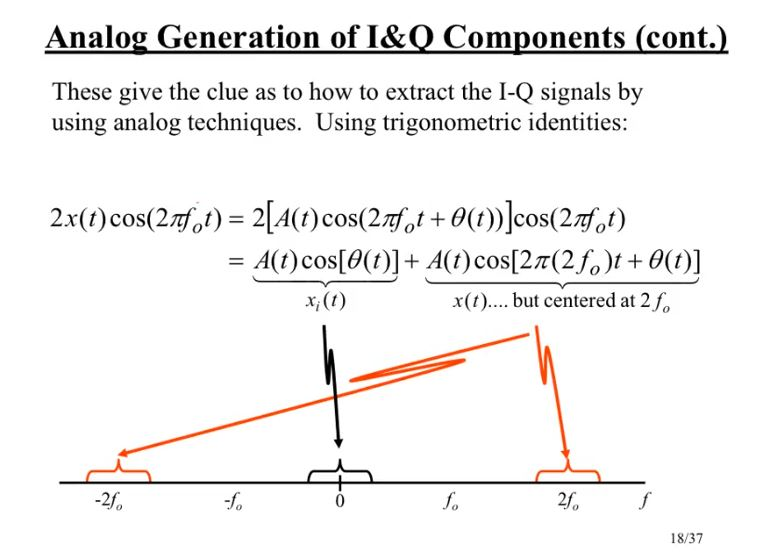
\includegraphics[width = 0.7\textwidth, frame]{Figures/Sampling/IQ_trigonometric_identities}
\caption{Inphase term generation }
\label{fig:Sampling:IQ_trigonometric_identities}
\end{figure}

\begin{itemize}

\item We use the trigonometric identities of the argument of a cos

\item Notice that we obtained the in-phase term, but with a high frequency component centered at $2\, f_{\text{ceneter}}$, so we need to use a low pass filter

\end{itemize}


\begin{figure}[h]
\centering
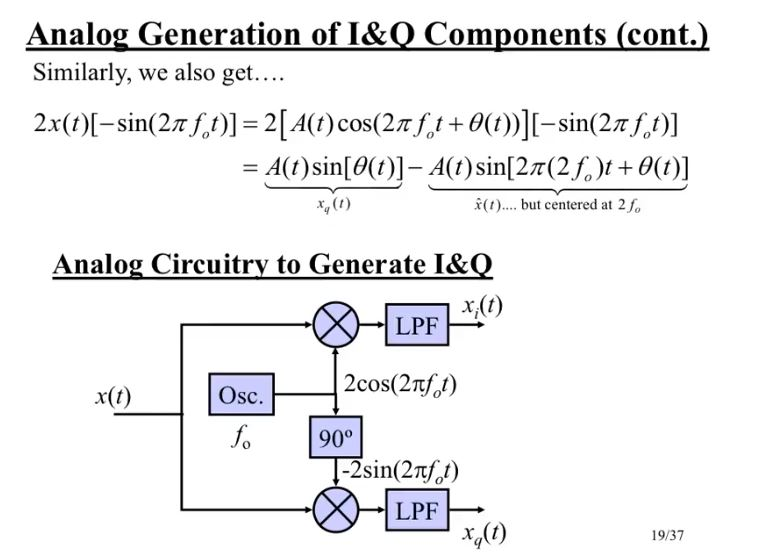
\includegraphics[width = 0.7\textwidth, frame]{Figures/Sampling/qudrature_impelmentation}
\caption{IQ generation and implementation using analog devices}
\label{fig:Sampling:qudrature_impelmentation}
\end{figure}

\begin{itemize}

\item The multiplication is a mixer and the phase shift is implemented using a phase shifter

\item The cos signal is generated using an oscillator

\end{itemize}

Also, the in-phase and quadarature components can be generated digitally, as shown in, using some DSP processor.

\begin{itemize}

\item Instead of a mixer, we can do multiplication numerically

\item Instead of an oscillator, we can do generate the cos numerically also

\end{itemize}


\section{Sampling Dilemma using I and Q Components}

Suppose we have generate the I and Q components and we want to process them in a system for some purpose. Usually, we put some ADC after the I and Q to do the processing in discrete time.\\

According to Shannon theorem, we need to sample twice as fast the highest frequency component, which is $B$ according to , if we take the $X_{\text{Eq-Baseband}}(f_c)$ amplitude spectrum.\\

However, the original band pass signal $X_{\text{Bandpas}}(f_c)$ has a bandwidth of $B$, so according to Shannon, we need to sample at $2 \, B$.

\begin{figure}[h]
\centering
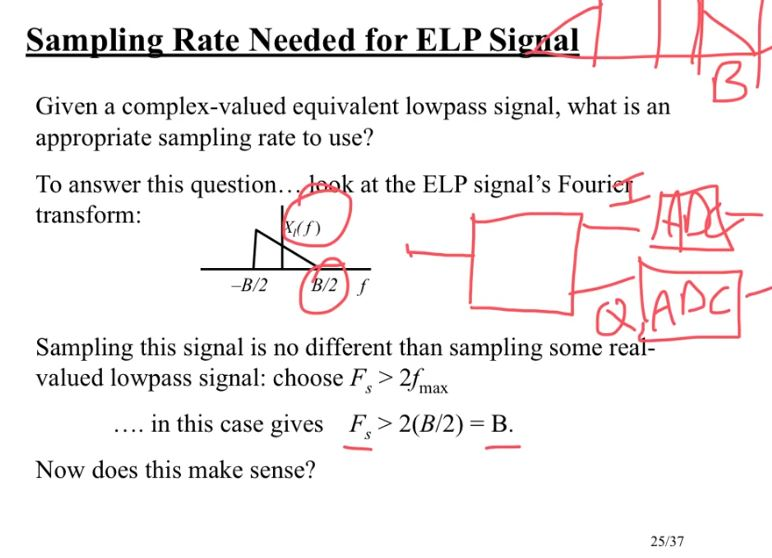
\includegraphics[width = 0.7\textwidth, frame]{Figures/Sampling/sampling_IQ}
\caption{IQ sampling}
\label{fig:Sampling:sampling_IQ}
\end{figure}

\newpage
But we need not to forget that $X_{\text{Eq-Baseband}}(f_c)$ is composed from 2 signals, and each signal is sampled at a rate of $B$, which make sense.

\begin{figure}[h]
\centering
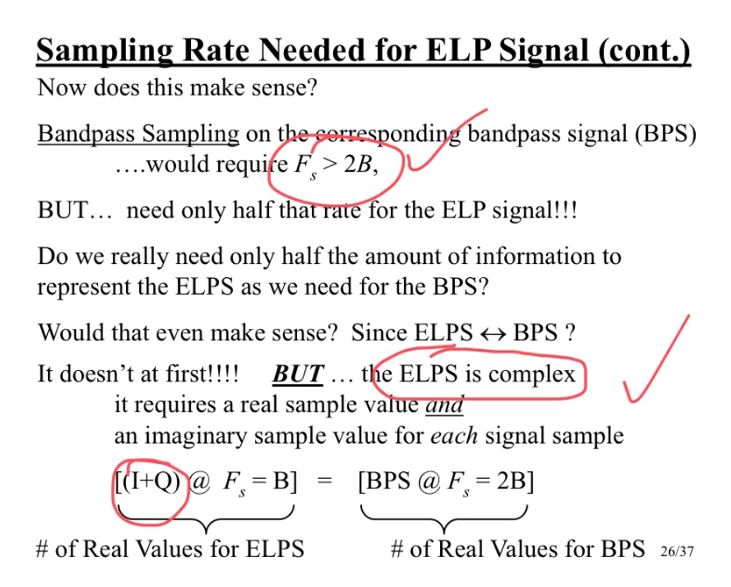
\includegraphics[width = 0.7\textwidth, frame]{Figures/Sampling/sampling_IQ_2}
\caption{IQ sampling: each component is sampled at a rate of $B$}
\label{fig:Sampling:sampling_IQ_2}
\end{figure}


\newpage
\subsection{Integer band positioning}


\begin{figure}[h]
\centering
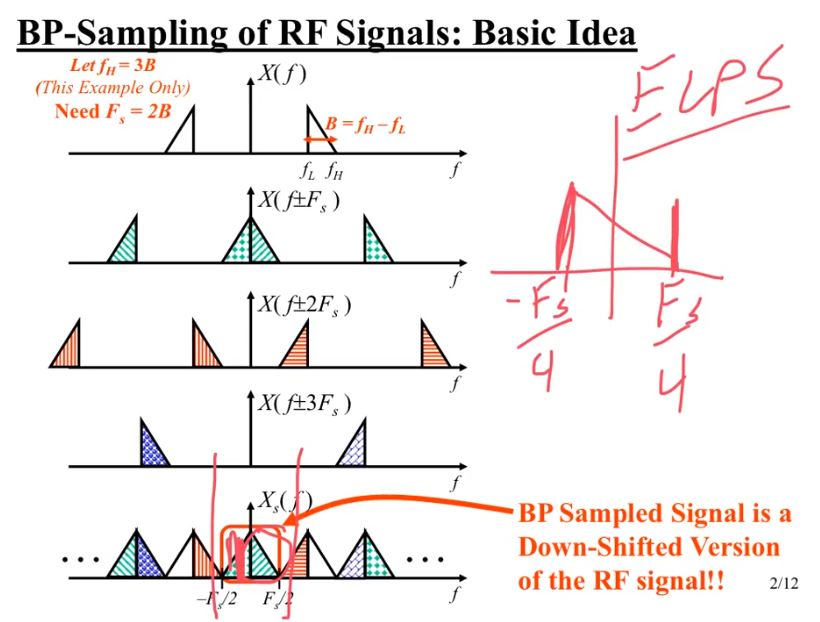
\includegraphics[width = 0.7\textwidth, frame]{Figures/Sampling/bandpass_sampling_ex_1}
\caption{Bandpass sampling example 1}
\label{fig:Sampling:bandpass_sampling_ex_1}
\end{figure}

\begin{itemize}

\item We have a bandpass signal of bandwidth $B$ and $f_{\text{high}} \, = \, 3B$

\item The theory tells us that we need to sample at twice the maximum frequency in the signal, so $F_s \, = \, 6B$


\item However, in the example of \autoref{fig:Sampling:bandpass_sampling_ex_1}, we sample at $F_s \, = \, 2B$


\item When we sample $F_s \, = \, 2B$, the theory tells to add the replicate of the spectrum at multiple of $F_s$

	\begin{itemize}
	\item Each portion of the spectrum (positive and negative) will be shifted at multiple of $F_s$
	\end{itemize}


\item At the end we obtain $X_{\text{sampled}}(f_c)$

	\begin{itemize}

	\item To reconstruct the bandpass signal, we low pass the signal then shifted to obtain the equivalent base band signal
	
	
	\end{itemize}



\end{itemize}


\newpage
\underline{General Case:}\\


\begin{figure}[h]
\centering
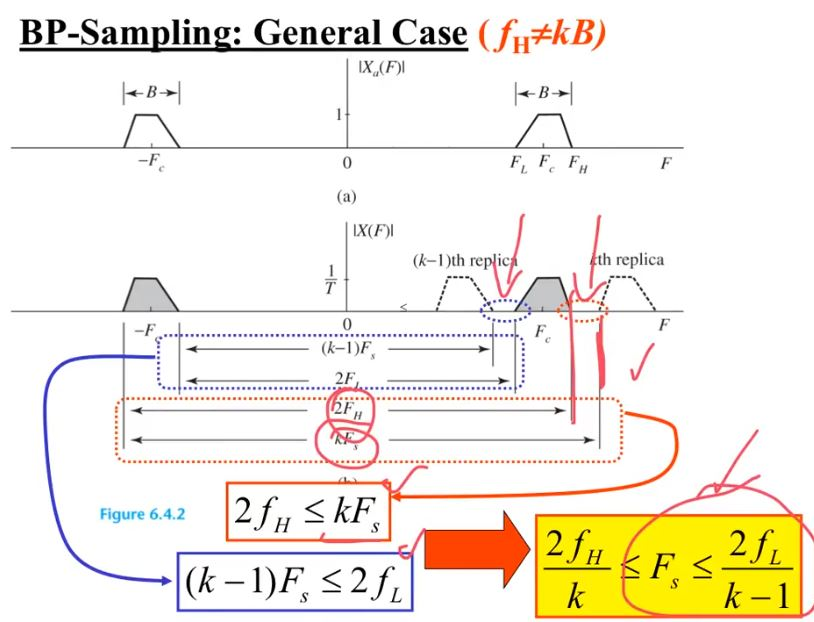
\includegraphics[width = 0.7\textwidth, frame]{Figures/Sampling/bandpass_sampling_general_case_non_integer}
\caption{Bandpass sampling non integer case}
\label{fig:Sampling:bandpass_sampling_general_case_non_integer}
\end{figure}

\begin{itemize}

\item We want that the images don't overlap with the original spectrum of the bandpass signal

\item The 2 inequality contstraints comes from $f_{\text{low}}$ and $f_{\text{high}}$

\item The larger $k$ we have, the lower $F_s$ we can choose.

	\begin{itemize}
	\item However, we don't have an idea about $k$ yet
	\end{itemize}

\newpage
\item Now we formulate a bound on $k$ shown in \autoref{fig:Sampling:bandpass_sampling_general_case_non_integer_bound_k}.


\begin{figure}[h]
\centering
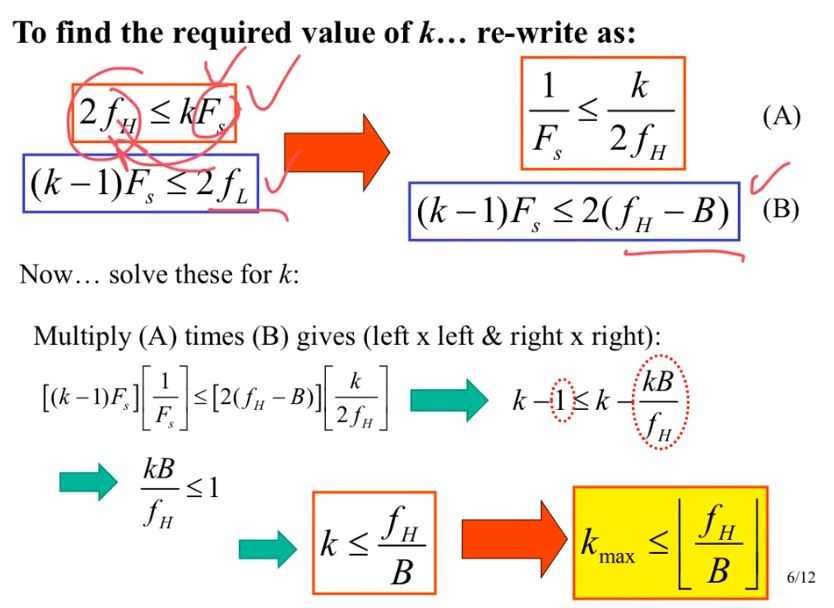
\includegraphics[width = 0.7\textwidth, frame]{Figures/Sampling/bandpass_sampling_general_case_non_integer_bound_k}
\caption{Bandpass sampling non integer case: bounding $k$}
\label{fig:Sampling:bandpass_sampling_general_case_non_integer_bound_k}
\end{figure}


\item As summary:

\begin{equation}
\begin{array}{rcl}
\displaystyle\frac{2 \, f_{\text{high}}}{k} \, &\leq& \, F_s \,\, \, \, \leq \, \displaystyle\frac{2 \,\left( \,  f_{\text{high}} \, - \, \text{Bandwidth} \, \right)}{k \, - \, 1} \\ \\
k \, &\leq& \, \displaystyle\frac{2 \, f_{\text{high}}}{\text{Bandwidth}} 
\end{array}
\label{Eq:Sampling:bandpass_sampling_bounds}
\end{equation}

\newpage
Plotting equations (\ref{Eq:Sampling:bandpass_sampling_bounds}) give us plot shown in \autoref{fig:Sampling:bandpass_sampling_general_case_plots}.


\begin{figure}[h]
\centering
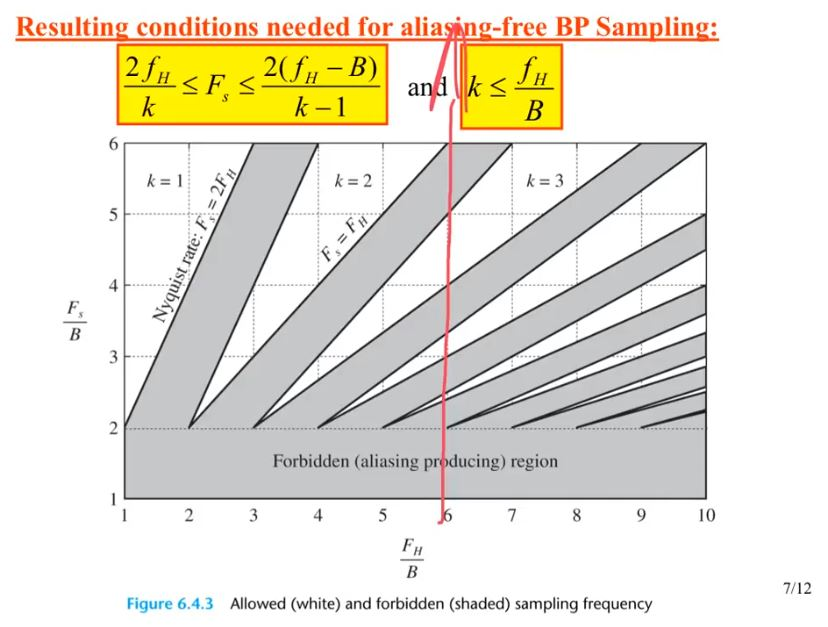
\includegraphics[width = 0.7\textwidth, frame]{Figures/Sampling/bandpass_sampling_general_case_plots}
\caption{Bandpass sampling plot: $F_s$ function of $f_{\text{high}}$}
\label{fig:Sampling:bandpass_sampling_general_case_plots}
\end{figure}

	\begin{itemize}
	\item The plots are normalized over the bandwidth $B$, which makes plotting the equation more easy
	
	\item $k \, = \, 1$: we are operating on the standard Nyquiste rate
	
	
	\item if we have $\displaystyle\frac{f_{\text{high}}}{\text{ bandwidth}} \, = \, 6$, we can operate at multiple $k$: 1,2, 3 and 4 and even 5 (the higher $k$ the lower is $F_s$)
	
	\newpage
	\item However, we have to pay attention at $k \, = \, 5$
	
	\begin{figure}[h]
\centering
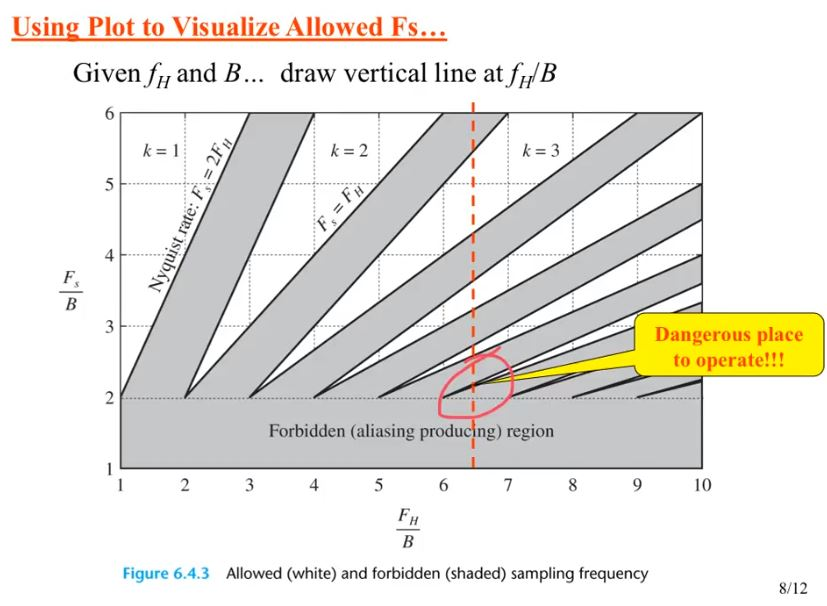
\includegraphics[width = 0.7\textwidth, frame]{Figures/Sampling/bandpass_sampling_general_case_plots_2}
\caption{Bandpass sampling plot: dangerous area we need to pay attention from}
\label{fig:Sampling:bandpass_sampling_general_case_plots_2}
\end{figure}

	\item From this dangerous place, comes the idea of guard band shown in \autoref{fig:Sampling:bandpass_sampling_guard_bands}
	
	
	\begin{figure}[h]
\centering
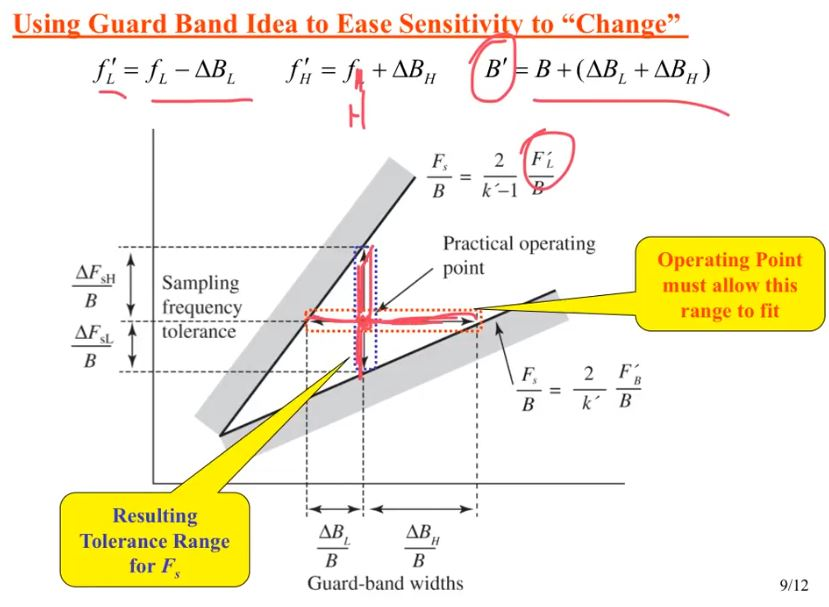
\includegraphics[width = 0.7\textwidth, frame]{Figures/Sampling/bandpass_sampling_guard_bands}
\caption{Bandpass sampling plot:putting some guard bands}
\label{fig:Sampling:bandpass_sampling_guard_bands}
\end{figure}
	
	\end{itemize}

\end{itemize}